\documentclass[twoside]{article}

\usepackage{aistats2027}
% For the camera-ready version use \usepackage[accepted]{aistats2027};
% for a non-anonymous preprint use \usepackage[preprint]{aistats2027}.

% Author-year citations (required for camera-ready).
\usepackage[round]{natbib}
\renewcommand{\bibname}{References}
\renewcommand{\bibsection}{\subsubsection*{\bibname}}
\bibliographystyle{apalike}

\usepackage[hyphens]{url}
\usepackage{graphicx}
\usepackage{amssymb}
\usepackage{booktabs}
\usepackage{multirow}

% Figures live in ../resources/ (shared with the other paper versions).
\graphicspath{{../}}

\begin{document}

\runningtitle{Band Depth Uncertainty Quantification for Chain-of-Thought Reasoning}
\runningauthor{Anonymous Authors}

\twocolumn[

\aistatstitle{Band Depth Uncertainty Quantification for Chain-of-Thought Reasoning via Embedded Reasoning Graphs}

\aistatsauthor{ Anonymous Author(s) }

\aistatsaddress{ Anonymous Institution } ]

\begin{abstract}
Chain-of-Thought (CoT) reasoning shows how a large language model reaches its
answer, not just the answer itself. Yet black-box uncertainty quantification (UQ)
methods largely ignore this reasoning and rely on agreement among final answers. Chains that reach the same
answer through different reasoning are not equally trustworthy, but answer-level
consistency cannot tell them apart. We argue that uncertainty lies in the
\emph{geometry} of the reasoning: how central each chain is within the ensemble.
We propose \textbf{BD-UQ}, a family of black-box UQ methods that measure this
centrality with \emph{band depth}, a notion from functional data analysis, applied
to a reasoning graph built from sampled chains. BD-UQ needs only a small sentence
encoder and no additional LLM calls, and across five benchmarks and four LLMs it
consistently outperforms sampling-based and verbalized baselines.
\end{abstract}

% -----------------------------------------------------------------------
\section{Introduction}
\label{sec:intro}

\begin{figure*}[t]
  \centering
  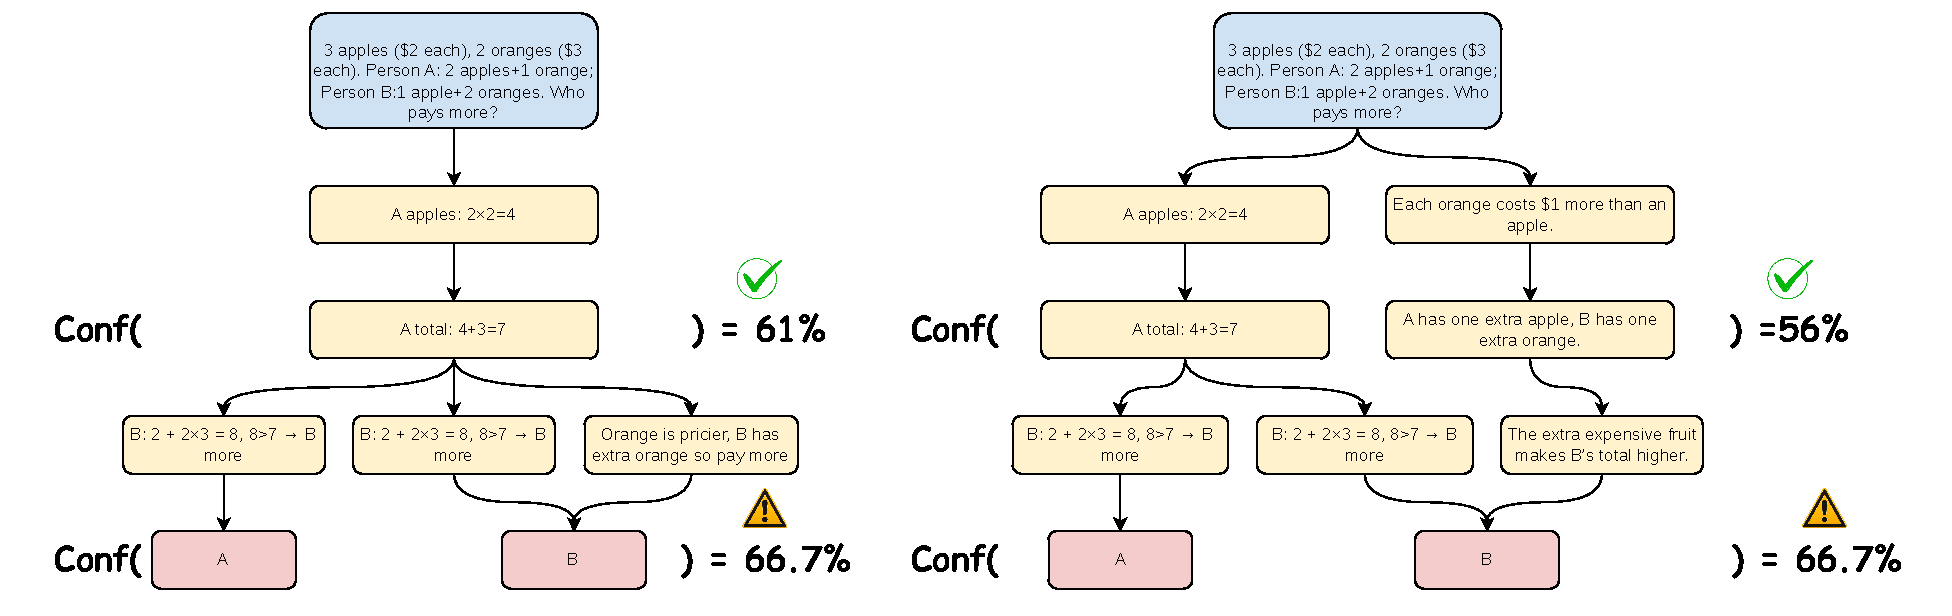
\includegraphics[width=0.95\textwidth]{resources/intro_motivation}
  \caption{Answer-level versus reasoning-level uncertainty. Two ensembles of three
  CoT responses share the same answer split (two $B$, one $A$), so answer-level
  agreement gives both the same confidence ($\mathrm{Conf(ans)}=66.7\%$). The chains
  on the left diverge only at the \emph{final} step, those on the right diverge
  \emph{early}; reasoning-level confidence separates the two
  ($\mathrm{Conf(CoT)}=61\%$ vs.\ $46\%$).}
  \label{fig:intro}
\end{figure*}

Large language models have become capable general-purpose reasoners, in
large part due to Chain-of-Thought prompting~\citep{wei2022chain}, which
elicits explicit step-by-step reasoning before a final answer and has driven
strong gains on mathematical and multi-hop reasoning tasks~\citep{wang2023selfconsistency, yao2023tree}.
As these models are deployed in increasingly consequential settings, however,
their fluent but sometimes confidently wrong outputs make it essential to know
\emph{when to trust} a given response. Uncertainty quantification addresses
this by attaching a confidence score to each generation, ideally one that ranks
correct answers above incorrect ones. The most practically important regime is
\emph{black-box} UQ, where only the generated text is available---no token
logits, hidden states, or gradients---since this is the only access mode offered
by the strongest proprietary models and the cheapest to deploy for open ones.

Existing black-box UQ methods almost universally reduce a response to its
\emph{final answer} and measure agreement across multiple sampled answers.
Self-consistency counts how often the majority answer recurs~\citep{wang2023selfconsistency};
semantic entropy clusters answers by meaning and measures the entropy of the
cluster distribution~\citep{kuhn2023semantic, farquhar2024detecting};
and related approaches compute pairwise answer similarity or
non-contradiction~\citep{lin2023generating, manakul2023selfcheckgpt, chen2024quantifying}.
A second line of work instead asks the model to \emph{verbalize} its own
confidence, either directly or by self-probing in a fresh
context~\citep{xiong2024llms, liu2024uait}. Both families have a common
blind spot: they treat the reasoning chain---the very structure CoT was designed
to produce---as a black box. Answer-level methods discard it entirely, and
verbalized methods rely on the model's unreliable introspection over it.



This blind spot matters because the reasoning chain carries information that the
final answer cannot. As illustrated in Figure~\ref{fig:intro}, two responses may
converge on the same answer through entirely different reasoning paths---one
sound, one a lucky coincidence of errors---yet answer-level consistency assigns
them identical confidence.
Conversely, an ensemble whose chains disagree sharply at intermediate steps
signals genuine model uncertainty even when the final answers happen to match.
Recent work has begun to incorporate reasoning into UQ: CoT-UQ extracts
keywords and importance scores from each step to reweight token
probabilities~\citep{zhang2025cotuq}, and graph-based metrics summarize
relationships among extracted claims~\citep{jiang2024graphuncertainty}. Yet
CoT-UQ still requires token logits (and is therefore not fully black-box) and
operates on a single response rather than an ensemble, while claim-graph methods
target long-form factuality rather than the geometry of reasoning itself. The
question of how to extract uncertainty from the \emph{structure} of an ensemble
of reasoning chains, using text alone, remains open.

We argue that the right signal lives in the \emph{geometry} of the reasoning
ensemble: where chains converge, where they diverge, and how central each chain
is relative to the others. To capture this, we turn to \emph{band depth}, a
concept from functional data analysis that ranks a set of curves from most
central (the functional median) to most outlying~\citep{lopezpintado2009banddepth},
and which has been extended to ensembles of contours and of paths on a
graph~\citep{santer2023contourbanddepth, raj2017pathboxplots}. Building on this
lineage, we embed every reasoning step of every sampled chain with a sentence
encoder~\citep{reimers2019sentencebert} and construct a \emph{reasoning graph}
whose nodes are semantic clusters of steps and whose edges encode sequential and
cross-chain proximity. On this graph we define a family of depth-based
confidence scores---\textbf{pBD}, \textbf{vBD}, and \textbf{gBD}---that measure
how central each chain is within the ensemble. A chain that lies deep inside the
ensemble's reasoning band is trustworthy; an outlying chain is not. Crucially,
all variants are fully black-box and model-free: they require only the sampled
text and a lightweight encoder, with no additional LLM calls.

Our contributions are as follows:
\begin{itemize}
  \item \textbf{Conceptually}, we identify the structure of CoT reasoning
        ensembles as an untapped source of black-box uncertainty, and show that
        the geometric notion of band depth provides a principled way to exploit
        it---going beyond both answer-level consistency and verbalized
        self-probing.
  \item \textbf{Technically}, we introduce a reasoning-graph construction over
        sampled CoT chains and three band-depth confidence estimators on it:
        \textbf{pBD} (path-level, order-sensitive), \textbf{vBD} (vertex-level,
        order-invariant), and \textbf{gBD} (path-level via random walks,
        order-invariant), each requiring no token logits and no extra LLM
        inference.
  \item \textbf{Empirically}, we evaluate on five benchmarks across mathematical
        reasoning~\citep{cobbe2021gsm8k, patel2021svamp, miao2020asdiv} and
        multi-hop question answering~\citep{yang2018hotpotqa, ho2020wikimultihop}
        with three open-weight models across two families and
        scales~\citep{touvron2023llama2, grattafiori2024llama3, qwen2024qwen25},
        showing that gBD consistently and substantially outperforms
        sampling-based and verbalized baselines.
\end{itemize}

% -----------------------------------------------------------------------
\section{Preliminaries}
\label{sec:prelim}

\paragraph{Problem setup.}
Let $\mathcal{M}$ denote a black-box LLM: given a prompt $x$, it returns a
response $y \sim \mathcal{M}(\cdot \mid x)$, and we assume access only to its
generated text. For a dataset
$\{x_i\}_{i=1}^{N}$ with reference answers $\{y_i^\star\}_{i=1}^{N}$, an oracle
correctness function $h(y_i; y_i^\star) \in \{0, 1\}$ indicates whether response
$y_i$ is correct; this label is used only for offline evaluation and is
unavailable at inference time. The goal of UQ is to design a confidence scorer
\begin{equation}
  \hat{s}: y_i \mapsto \hat{s}(y_i)\in[0,1],
\end{equation}
that assigns higher scores to correct responses than to incorrect ones.
Because $\hat{s}$ depends only on model outputs and never on $y_i^\star$, it
serves as a practical proxy for the inaccessible oracle.

\paragraph{Chain-of-Thought generation.}
Under Chain-of-Thought prompting~\citep{wei2022chain}, a response is not a
bare answer but a structured reasoning trace. We write a CoT response as an
ordered sequence of reasoning steps followed by a final answer,
\begin{equation}
  y_i = (s_1, s_2, \ldots, s_k, a),
\end{equation}
where each $s_j$ is a natural-language reasoning step and $a$ is the extracted
final answer. Throughout, we refer to the step sequence
$P = (s_1, \ldots, s_k)$ as a \emph{reasoning chain} (or path) and to $a$ as its
answer.

\paragraph{Ensemble of reasoning chains.}
Rather than scoring a single response, our methods operate on an \emph{ensemble}
of CoT responses sampled for the same prompt. For each $x_i$, we draw $M$
responses under stochastic decoding,
\begin{equation}
  \{ y_i^{(1)}, \ldots, y_i^{(M)} \} \sim \mathcal{M}(\cdot \mid x_i),
  \qquad
  y_i^{(m)} = (P_i^{(m)}, a_i^{(m)}),
\end{equation}
yielding $M$ reasoning chains $\{P_i^{(m)}\}_{m=1}^{M}$ and their answers
$\{a_i^{(m)}\}_{m=1}^{M}$. Answer-level baselines summarize only the multiset of
answers $\{a_i^{(m)}\}$; in contrast, our methods (Section~\ref{sec:method})
exploit the full set of chains $\{P_i^{(m)}\}$. We embed each reasoning step with
a frozen sentence encoder~\citep{reimers2019sentencebert}, mapping a step $s$ to
a vector $e(s) \in \mathbb{R}^d$, which provides the geometric substrate on
which band depth is computed.

\paragraph{Evaluation metric.}
Following standard practice in LLM UQ~\citep{kuhn2023semantic, xiong2024llms}, we
evaluate confidence scorers by the Area Under the Receiver Operating
Characteristic curve (AUROC) between the predicted scores $\{\hat{s}(y_i)\}$ and
the binary correctness labels $\{h(y_i; y_i^\star)\}$. AUROC measures the
probability that a randomly chosen correct response receives a higher confidence
than a randomly chosen incorrect one; a score of $1.0$ is perfect ranking and
$0.5$ corresponds to random guessing.

% -----------------------------------------------------------------------
\section{Methodology}
\label{sec:method}

\begin{figure*}[t]
  \centering
  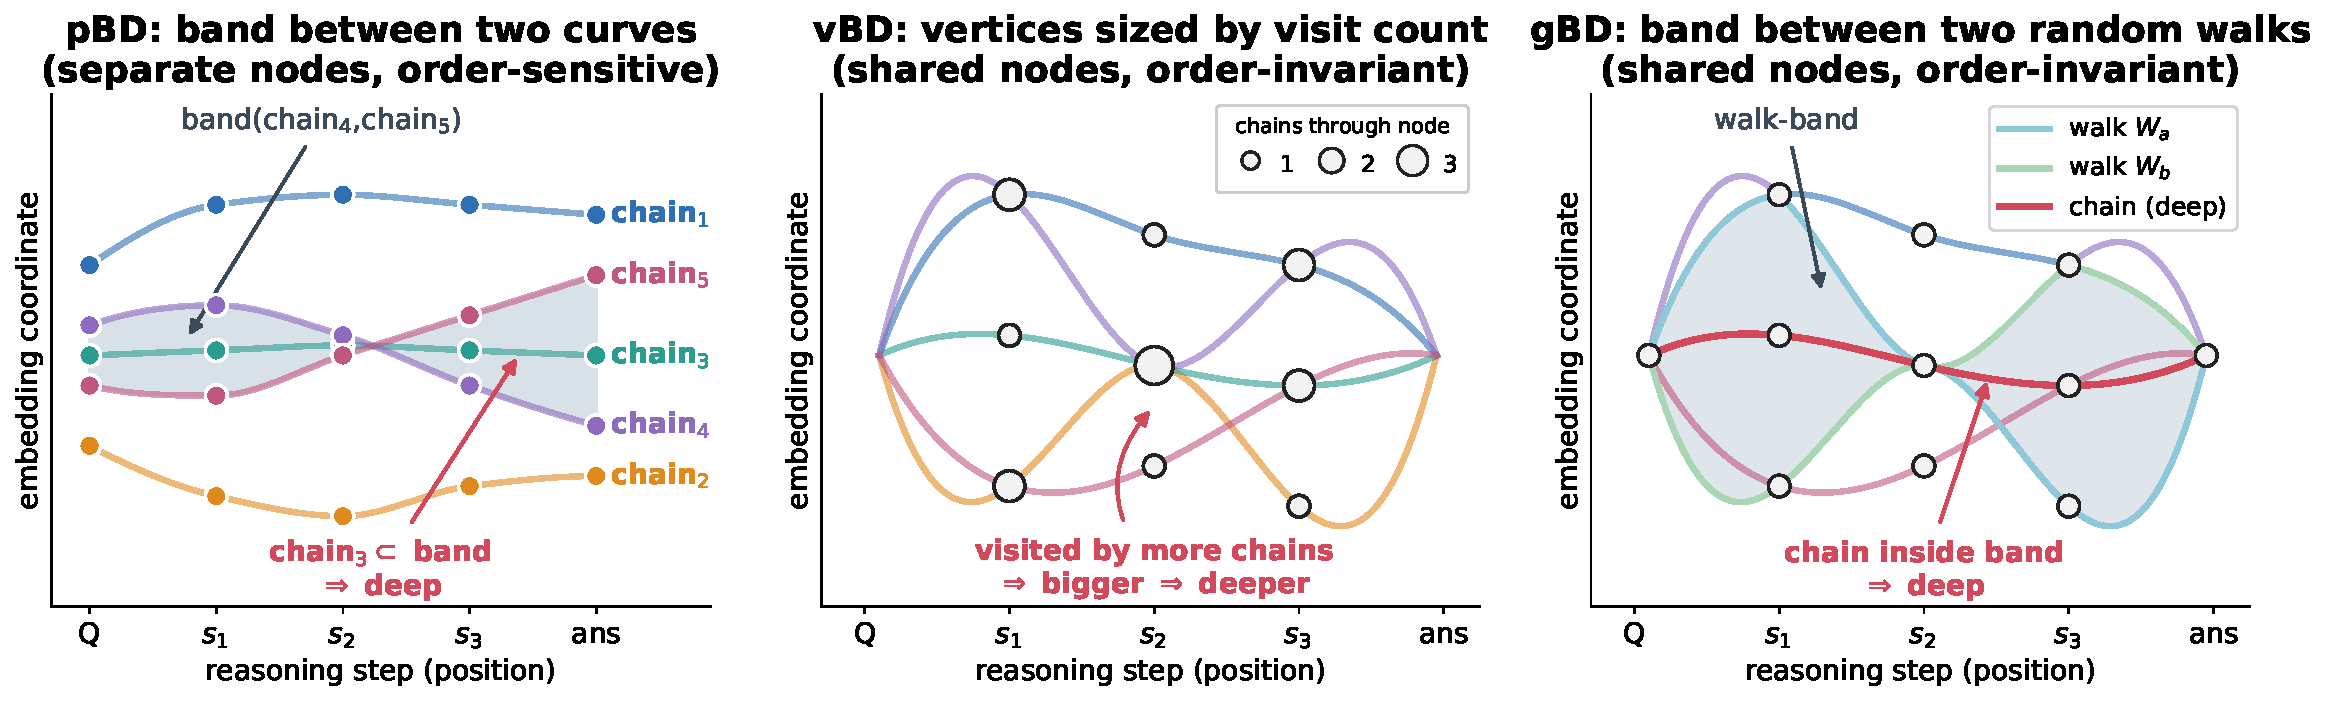
\includegraphics[width=0.95\textwidth]{resources/methods_overview}
  \caption{The three band-depth estimators, viewed as bands of curves. Each curve
  is one sampled CoT chain and each circle a reasoning step; a chain is \emph{deep}
  when it lies inside the bands formed by the other chains and \emph{shallow}
  otherwise. \textbf{pBD} compares position-aligned chains ($\mathrm{chain}_3$ lies
  within $\mathrm{band}(\mathrm{chain}_4,\mathrm{chain}_5)$) and is order-sensitive.
  \textbf{vBD} merges equivalent steps into shared vertices and scores a chain by
  the depth of the vertices it visits. \textbf{gBD} forms bands from pairs of random
  walks ($W_a, W_b$) on the same graph. vBD and gBD are order-invariant.}
  \label{fig:methods}
\end{figure*}

We now develop a family of black-box confidence scorers that act on the ensemble
of reasoning chains $\{P_i^{(m)}\}_{m=1}^{M}$ defined in
Section~\ref{sec:prelim}. The common principle is \emph{centrality}: a reasoning
chain that lies deep within the ensemble---surrounded and ``enclosed'' by the
others---reflects a stable, well-supported line of reasoning, whereas an
outlying chain signals instability. We make this precise through band depth and
present three estimators of increasing structural sophistication: pBD
(Section~\ref{sec:method:pbd}), vBD (Section~\ref{sec:method:vbd}), and gBD
(Section~\ref{sec:method:gbd}). For brevity we drop the prompt index $i$ and
write the ensemble as $\{P^{(1)}, \ldots, P^{(M)}\}$, with $P^{(m)} = (s_1^{(m)},
\ldots, s_{n_m}^{(m)})$ and step embeddings $e(s_j^{(m)}) \in \mathbb{R}^d$.

\paragraph{Band depth.}
Band depth is a notion from functional data analysis that ranks a sample of
curves from most central to most outlying~\citep{lopezpintado2009banddepth}.
Given a set of curves, any pair (or larger subset) delimits a \emph{band}, and
the depth of a curve is the fraction of bands that fully contain it; the curve of
maximal depth is the functional median, and low-depth curves are outliers. The
concept has been extended to ensembles of contours~\citep{santer2023contourbanddepth}
and of paths on a graph~\citep{raj2017pathboxplots}. We adapt these ideas to
reasoning chains: each chain plays the role of a curve, and its depth within the
ensemble serves as a confidence signal---high ensemble depth indicates agreement
and reliability, low depth indicates dispersion and uncertainty.



\subsection{pBD: Path Band Depth}
\label{sec:method:pbd}

pBD treats each reasoning chain as an \emph{ordered} sequence of step embeddings
(the pBD panel of Figure~\ref{fig:methods}) and measures how close a chain runs
to the ensemble's central tendency at each position. Because chains have
different lengths and may reason at different
paces, we align them with Dynamic Time Warping (DTW) before comparison.

For a chain $P^{(m)}$ and every other chain $P^{(r)}$ ($r \neq m$), let
$\sigma_r$ be the DTW alignment mapping each step index $k$ of $P^{(m)}$ to its
corresponding index in $P^{(r)}$. At each step index $k$ we form the
\emph{aligned centroid} of the other chains' matched steps,
\begin{equation}
  \mu_k^{(m)} = \frac{1}{M-1} \sum_{r \neq m} e\big(s_{\sigma_r(k)}^{(r)}\big),
\end{equation}
and measure the \emph{centroid distance} $\delta_k^{(m)}$ of $s_k^{(m)}$ to that
centroid,
\begin{equation}
  \delta_k^{(m)} = 1 - \cos\!\big( e(s_k^{(m)}),\, \mu_k^{(m)} \big) \in [0, 1],
\end{equation}
so that a small $\delta_k^{(m)}$ means $s_k^{(m)}$ sits close to the ensemble's
consensus at position $k$. The path depth of $P^{(m)}$ is its mean closeness to
the centroids,
\begin{equation}
  s^{(m)} = \frac{1}{n_m} \sum_{k=1}^{n_m} \big( 1 - \delta_k^{(m)} \big),
\end{equation}
and the ensemble-mean depth $\bar{s} = \frac{1}{M} \sum_{m=1}^{M} s^{(m)}$ is
then combined with answer agreement to form the final confidence through the
shared blend of Eq.~\eqref{eq:blend}.

Despite capturing uncertainty in the CoT chain, pBD has its own weakness. In
Table~\ref{tab:ensemble-example}, two chains were produced for a single HotpotQA
question and both reach the correct answer ``We Are the Ocean'' through the same
four-step logic---look up each band's member count, compare the two numbers, and
conclude. The chains are identical in length and wording and differ \emph{only}
in the \emph{order} of the two member-count lookups: Chain~A states ``We Are the
Ocean'' first, Chain~B states ``The Dream Academy'' first. Conceptually the two
chains are the same, but pBD compares step embeddings position by position, so it
aligns ``We Are the Ocean has 5 members'' (Chain~A, step~1) against ``The Dream
Academy has 3 members'' (Chain~B, step~1) and registers large spurious diversity,
deflating the depth exactly where confidence should be highest. pBD is therefore
\emph{order-sensitive}, even though agreement among reasoning chains is inherently
order-invariant. Computationally, aligning every pair of chains with DTW costs
$O(n^2 d)$ per pair and $O(M^2 n^2 d)$ for the full ensemble. Both problems stem
from insisting on a position-wise, sequential view of the chains.

\begin{table}[t]
  \caption{Two Chain-of-Thought chains for the HotpotQA question
  \emph{``Which band has more members, We Are the Ocean or The Dream Academy?''}
  (WATO = We Are the Ocean, TDA = The Dream Academy). The chains differ
  \emph{only} in the order of steps 1--2, yet pBD's position-wise comparison counts
  them as diverse.}
  \label{tab:ensemble-example}
  \centering
  \footnotesize
  \setlength{\tabcolsep}{6pt}
  \begin{tabular}{c|ll}
    \toprule
    Step & \textbf{Chain A} & \textbf{Chain B} \\
    \midrule
    1 & WATO has 5 members & TDA has 3 members \\
    2 & TDA has 3 members  & WATO has 5 members \\
    3 & $5 > 3$            & $5 > 3$ \\
    4 & WATO is larger     & WATO is larger \\
    \bottomrule
  \end{tabular}
\end{table}

\subsection{Reasoning Graph Construction}
\label{sec:method:graph}

To mitigate both the order-sensitivity and the alignment cost of pBD, we abandon
position-wise comparison and instead collapse the ensemble into a single
\emph{reasoning graph} $G = (V, E)$, which is used later in vBD and gBD. By merging
semantically equivalent steps into shared nodes regardless of where they appear
in a chain, the graph maps the reordered lookups of
Table~\ref{tab:ensemble-example} onto one shared structure: equivalent reasoning
is no longer counted as diversity and no pairwise alignment is needed. Starting from the embedded steps of all $M$
chains:
\begin{itemize}
  \item \textbf{Nodes.} Steps whose pairwise cosine similarity exceeds a high
        threshold $\theta_c$ are merged into a single node, so that each
        $v \in V$ represents a semantic cluster of equivalent reasoning states.
  \item \textbf{Sequential edges.} Consecutive steps within the same chain are
        joined by a directed edge, preserving local reasoning flow.
  \item \textbf{Semantic edges.} Steps from different chains whose cosine
        similarity exceeds a lower threshold $\theta_e < \theta_c$ are joined by
        an undirected edge, linking related reasoning across chains.
\end{itemize}
Each reasoning chain $P^{(m)}$ thereby becomes a walk over $V$, and the geometry
of the ensemble is encoded in the topology of $G$.

\subsection{vBD: Vertex Band Depth}
\label{sec:method:vbd}

vBD measures the \emph{centrality of each individual vertex} in the reasoning
graph (the vBD panel of Figure~\ref{fig:methods}), and then scores a chain by how
central the nodes it visits are. A vertex is central if it lies ``between'' many other reasoning
states---a node that the bulk of the graph encloses---and peripheral if it sits
at the fringe. Because
only the \emph{set} of visited nodes enters the score, vBD is fully
order-invariant. Concretely, we sample vertex pairs uniformly from the vertex set $V$. For a
vertex $v$, its vertex band depth is the probability that $v$ lies inside the
geodesic convex hull $H[\cdot]$ of two vertices
$\mathcal{V}_2 = \{v_a, v_b\}$ drawn at random from $V$,
\begin{equation}
  v\text{BD}(v) = \mathbb{E}_{\mathcal{V}_2 \sim V}\!\left[ \mathbf{1}\big(v \in H[\mathcal{V}_2]\big) \right],
\end{equation}
estimated by Monte Carlo sampling of $S$ such pairs from $V$. The depth of a
chain is the mean vertex depth over the nodes it visits,
\begin{equation}
  v\text{BD}\big(P^{(m)}\big) = \frac{1}{|P^{(m)}|} \sum_{v \in P^{(m)}} v\text{BD}(v),
\end{equation}
and the ensemble-mean depth $\bar{s} = \frac{1}{M} \sum_{m=1}^{M} v\text{BD}(P^{(m)})$
again enters the shared confidence blend of Eq.~\eqref{eq:blend}.

Beyond graph construction, vBD requires only $S$ sampled vertex pairs from $V$,
each needing a geodesic-hull membership test, and is far cheaper than pBD's
pairwise DTW. Its limitation is that it treats each vertex \emph{independently}:
by averaging per-vertex depths it ignores how those vertices are linked into a
path---the transitions a chain takes and the order in which it visits states.
Two chains that occupy the same set of central nodes but connect them through
very different reasoning receive the same vBD score, even if one follows a
coherent route through the graph and the other jumps erratically between
unrelated states. vBD thus captures \emph{which} reasoning states a chain
occupies but not \emph{how} it moves among them.

\subsection{gBD: Graph Band Depth}
\label{sec:method:gbd}

gBD, our main method, returns depth to the \emph{path} level while remaining
order-invariant, recovering exactly the information vBD discards: the relations
between steps---which reasoning states follow which, and how a chain threads them
together. Whereas vBD asks only whether a chain's individual nodes are central,
gBD asks whether the chain's whole \emph{trajectory} through the graph is central.
A chain that visits central nodes but connects them through incoherent jumps is
no longer scored as though it reasoned coherently, because its transitions, not
just its nodes, are evaluated.

gBD also differs fundamentally from pBD in its \emph{reference distribution}. pBD
can compare only the $M$ chains the model actually sampled, aligned pairwise; it
never considers any reasoning beyond those $M$. Our graph, by contrast, clusters
semantically equivalent steps into shared nodes and links steps across chains
with edges, so it encodes reasoning transitions that no \emph{single} sampled
chain exhibits, and random walks on $G$ synthesize new chains from them. Using such
walks as reference paths (the gBD panel of Figure~\ref{fig:methods}), gBD measures
a chain's depth against the full reasoning space the graph defines rather than only
the $M$ observed chains, which keeps the estimate robust when the ensemble is small.

For each real chain $P^{(m)}$ we draw $T$ pairs of random walks
$(W_a^{(t)}, W_b^{(t)})$ on $G$ and measure the fraction of $P^{(m)}$'s vertices
that fall inside the geodesic convex hull of each pair (soft containment),
averaged over the $T$ draws,
\begin{equation}
  \text{gBD}\big(P^{(m)}\big) = \frac{1}{T} \sum_{t=1}^{T}
  \frac{\big|\{\, v \in P^{(m)} : v \in H_t \,\}\big|}{|P^{(m)}|},
\end{equation}
where $H_t = \text{hull}(W_a^{(t)}, W_b^{(t)})$.
The final confidence blends the mean depth $\bar{s}$ with the answer-level
majority fraction $\rho$ (the share of chains agreeing with the modal answer),
\begin{equation}
\label{eq:blend}
  \hat{s} = \alpha \, \bar{s} + (1 - \alpha)\, \rho.
\end{equation}
For gBD $\bar{s} = \overline{\text{gBD}} = \frac{1}{M}\sum_m \text{gBD}(P^{(m)})$,
and the same form of blend is applied to all three estimators, substituting the
corresponding depth score $\bar{s}$ of pBD or vBD. We consider two variants for generating
the reference walks:
\begin{itemize}
  \item \textbf{gBD-v1 (anchored):} walks are constrained to start at the graph's
        input node and end at its output node, following the global
        question-to-answer direction.
  \item \textbf{gBD-v2 (free):} walks may start and end anywhere in $G$, freely
        exploring its topology; this is our strongest estimator.
\end{itemize}

gBD draws $T$ walk pairs per chain and performs hull-membership tests, comparable
in cost to vBD and far below pBD.

% -----------------------------------------------------------------------
\section{Related Works}
\label{sec:related}

\subsection{Black-box Uncertainty Quantification for LLMs}
Most black-box methods score the consistency of multiple sampled responses:
self-consistency uses majority-answer agreement~\citep{wang2023selfconsistency},
semantic entropy clusters responses by meaning~\citep{kuhn2023semantic, farquhar2024detecting},
and related work uses pairwise similarity or non-contradiction
rates~\citep{lin2023generating, manakul2023selfcheckgpt}, sampling-based
calibration~\citep{chen2024quantifying}, or selective
abstention~\citep{stelmakh2022selectively}. A complementary line elicits verbalized
confidence, which prompting studies find markedly overconfident~\citep{xiong2024llms}
and instruction tuning partially calibrates~\citep{liu2024uait}. Further approaches
use multi-agent interaction~\citep{feng2025multiagent}, iterative
prompting~\citep{abbasiyadkori2024believe}, or interrogative probing of long-form
outputs~\citep{fan2026iuq}.

Closer to us, CoT-UQ reweights token probabilities by step-keyword
importance~\citep{zhang2025cotuq} but needs logits and scores a single response,
and graph-based metrics over extracted claims~\citep{jiang2024graphuncertainty}
target long-form factuality. Cross-Model Disagreement~\citep{hamidieh2026crossmodel}
shares our diagnosis that self-consistency misses confidently wrong models, but
recovers the missing signal by querying \emph{other models}; we instead recover it
from the geometry of a single model's own reasoning ensemble. None of these methods
characterizes the \emph{structural centrality} of an ensemble of reasoning chains,
which is the signal our fully black-box methods exploit.

\subsection{Band Depth and Contour Ensembles}
Our geometric tools originate in functional data analysis, where band depth
provides a center-outward ordering of curves and identifies a functional
median~\citep{lopezpintado2009banddepth}. A substantial body of visualization
research has since extended depth to spatial ensembles. \textbf{Contour band depth}
generalizes the notion to ensembles of contours and underlies box-and-whisker
style summaries of two-dimensional uncertainty~\citep{santer2023contourbanddepth};
\textbf{inclusion depth} offers an efficient alternative based on inside/outside
relationships between contours~\citep{chavesdeplaza2024inclusiondepth}, and
further work handles multi-modal ensembles by disentangling their modes of
variation~\citep{chavesdeplaza2024multimodal}. Most relevant to us, band depth has
been generalized to ensembles of \emph{paths on a graph}, yielding a
center-outward ordering of paths and a corresponding \textbf{path
boxplot}~\citep{raj2017pathboxplots}. We build directly on this path-on-graph
formulation, but repurpose it: rather than visualizing ensemble uncertainty, we
treat the sampled reasoning chains of an LLM as the path ensemble and use their
depth as a black-box confidence score. To our knowledge, this is the first
application of band depth to LLM reasoning for uncertainty quantification.

% -----------------------------------------------------------------------
\section{Experiments}
\label{sec:exp}

\begin{table*}[t]
  \caption{AUROC ($\times 100$, $\uparrow$) for black-box UQ on five reasoning
  benchmarks. Best result per column (within a model) is in \textbf{bold}.}
  \label{tab:main-results}
  \centering
  \footnotesize
  \setlength{\tabcolsep}{6pt}
  \begin{tabular}{c l cc ccc}
    \toprule
    \multirow{2}{*}{\textbf{Model}} & \multirow{2}{*}{\textbf{Method}}
      & \multicolumn{2}{c}{\textbf{Multi-hop QA}}
      & \multicolumn{3}{c}{\textbf{Mathematical Reasoning}} \\
    \cmidrule(lr){3-4}\cmidrule(lr){5-7}
      & & HotpotQA & 2WikiMHQA & GSM8K & SVAMP & ASDiv \\
    \midrule
    \multirow{9}{*}{\textbf{Llama-3.1-8B}}
      & CoT-UQ                  & 54.92 & 56.67 & 54.58 & 54.35 & 51.77 \\
      & Non-Contradiction       & 58.62 & 58.54 & 57.49 & 64.34 & 66.40 \\
      & Entailment Prob.        & 63.78 & 58.32 & 63.72 & 69.22 & 72.41 \\
      & Semantic Entropy        & 62.33 & 52.98 & 60.80 & 62.82 & 67.05 \\
      & Cross-Model Disag.      & 73.69 & 63.30 & 61.86 & 57.92 & 64.47 \\
    \cmidrule(lr){2-7}
      & pBD                     & 76.29 & 62.31 & 65.99 & 69.49 & 72.61 \\
      & vBD                     & 76.16 & \textbf{69.22} & 64.90 & 67.14 & 69.77 \\
      & gBD-v1                  & 77.05 & 67.73 & 68.08 & 74.76 & 76.02 \\
      & gBD-v2                  & \textbf{77.19} & 68.39 & \textbf{68.69} & \textbf{74.81} & \textbf{76.12} \\
    \midrule
    \multirow{9}{*}{\textbf{Llama-2-13B}}
      & CoT-UQ                  & 67.43 & 57.06 & 53.02 & 51.25 & 56.23 \\
      & Non-Contradiction       & 63.99 & 67.74 & 54.47 & 62.66 & 65.87 \\
      & Entailment Prob.        & 68.03 & 64.28 & 65.96 & 63.93 & 72.70 \\
      & Semantic Entropy        & 63.51 & 59.27 & 61.61 & 56.10 & 66.00 \\
      & Cross-Model Disag.      & 70.93 & 68.01 & 65.93 & 61.57 & 71.29 \\
    \cmidrule(lr){2-7}
      & pBD                     & 74.83 & 62.64 & 72.29 & 67.60 & 74.41 \\
      & vBD                     & 73.84 & \textbf{73.60} & 69.47 & 66.22 & 71.40 \\
      & gBD-v1                  & 77.76 & 73.24 & 72.86 & 70.53 & 76.22 \\
      & gBD-v2                  & \textbf{78.04} & 73.12 & \textbf{73.13} & \textbf{70.74} & \textbf{76.51} \\
    \midrule
    \multirow{9}{*}{\textbf{Qwen2.5-3B}}
      & CoT-UQ                  & 67.22 & 58.62 & 57.98 & 65.45 & 64.38 \\
      & Non-Contradiction       & 46.71 & 47.13 & 60.88 & 65.99 & 62.79 \\
      & Entailment Prob.        & 58.77 & 54.98 & 61.19 & 66.55 & 67.54 \\
      & Semantic Entropy        & 55.75 & 57.40 & 65.32 & 69.06 & 57.29 \\
      & Cross-Model Disag.      & 75.32 & \textbf{72.67} & 65.31 & 63.24 & 68.02 \\
    \cmidrule(lr){2-7}
      & pBD                     & 76.83 & 62.60 & 60.35 & 70.58 & 67.38 \\
      & vBD                     & 76.70 & 66.28 & 60.01 & 70.52 & 64.71 \\
      & gBD-v1                  & 77.20 & 68.56 & 63.87 & \textbf{70.63} & 68.41 \\
      & gBD-v2                  & \textbf{78.59} & 66.65 & \textbf{65.40} & 70.27 & \textbf{68.56} \\
    \midrule
    \multirow{9}{*}{\textbf{Qwen3-8B}}
      & CoT-UQ      & 66.52 & 58.34 & 56.65 & 63.41 & 68.09 \\
      & Non-Contradiction       & 69.81 & 60.34 & 61.92 & 78.79 & 76.15 \\
      & Entailment Prob.        & 75.80 & 58.16 & 61.21 & 82.69 & 75.51 \\
      & Semantic Entropy        & 72.58 & 54.10 & 58.21 & 74.20 & 69.82 \\
      & Cross-Model Disag.      & 78.23 & 73.54 & 58.82 & 67.26 & 70.93 \\
    \cmidrule(lr){2-7}
      & pBD                     & 83.53 & 67.96 & 59.05 & 74.39 & 73.83 \\
      & vBD                     & 79.20 & \textbf{75.40} & 62.37 & 74.27 & 74.36 \\
      & gBD-v1                  & 84.64 & 75.35 & 70.15 & \textbf{86.31} & \textbf{84.18} \\
      & gBD-v2                  & \textbf{84.71} & 75.33 & \textbf{70.58} & 85.75 & 83.52 \\
    \bottomrule
  \end{tabular}
\end{table*}

\subsection{Experimental Setup}
\label{sec:exp:setup}

\textbf{Datasets.} We evaluate on five widely-used reasoning benchmarks chosen to
span two distinct regimes---closed-form mathematical reasoning and open-ended
multi-hop question answering---so that we can test whether band-depth scoring
generalizes across answer formats and correctness-grading protocols (exact match
vs.\ LLM grading) rather than exploiting a single task structure.
For mathematical reasoning we use GSM8K~\citep{cobbe2021gsm8k},
SVAMP~\citep{patel2021svamp}, and ASDiv~\citep{miao2020asdiv}, where correctness
is determined by exact match against the gold numerical answer. For multi-hop
question answering we use HotpotQA~\citep{yang2018hotpotqa} and
2WikiMultihopQA~\citep{ho2020wikimultihop}; following common practice for
open-ended answers, correctness is judged by an LLM grader. For 2WikiMultihopQA
we restrict to the \emph{inference} question type.

\textbf{Models.} We use four open-weight backbones spanning two families and a
range of scales: Llama-3.1-8B~\citep{grattafiori2024llama3},
Llama-2-13B~\citep{touvron2023llama2},
Qwen2.5-3B~\citep{qwen2024qwen25}, and Qwen3-8B~\citep{qwen2025qwen3}, applying
the same step-wise CoT prompt to all
four. For every question we sample an ensemble of $M = 5$ reasoning chains under
temperature decoding, which forms the common input to all ensemble-based scorers.

\textbf{Baselines.} We compare against two families of black-box scorers. The
first is \emph{CoT-UQ}~\citep{zhang2025cotuq}, a verbalized self-probing
method~\citep{xiong2024llms} in which the model is asked to state the probability
that its own answer is correct. It has five prompting variants---the vanilla
probe and four reasoning-augmented forms that condition on extracted keywords
(\textsc{KeyWords}, \textsc{AllKeyWords}) or reasoning steps (\textsc{KeyStep},
\textsc{AllStep})---of which we report the best-performing variant per dataset as
a single \textsc{CoT-UQ} entry. The second family is
\emph{sampling-based consistency}, which scores the ensemble by answer agreement:
Non-Contradiction probability and Entailment probability, both computed with an
NLI model, and Semantic Entropy~\citep{kuhn2023semantic, farquhar2024detecting}.
We additionally compare against \emph{Cross-Model Disagreement}
(CMD)~\citep{hamidieh2026crossmodel}, instantiated leave-one-out: for each
reference model the remaining three serve as the auxiliary ensemble, each with five
sampled responses. This spans two model families rather than the original five, so
our CMD numbers are a faithful-in-spirit rather than exact reproduction.

\textbf{Our methods and encoder.} We report all four band-depth estimators---pBD,
vBD, gBD-v1, and gBD-v2---computed on the same ensemble. Reasoning steps are
embedded with the all-MiniLM-L6-v2 sentence encoder~\citep{reimers2019sentencebert};
the graph-depth blending weight is fixed to $\alpha = 0.3$, the graph similarity
thresholds to $\theta_c = 0.92$ and $\theta_e = 0.70$, the band subset size to
$J = 2$, and the Monte-Carlo walk count to $T = 200$, all held constant across
datasets. None of our methods issue any LLM call beyond the initial ensemble.
Anonymized code is available at
\url{https://anonymous.4open.science/r/bd-uq-6F71/README.md}.
All LLM inference runs on an internal cluster of NVIDIA RTX A5500 GPUs (Ampere,
24\,GB, 10{,}240 CUDA cores), using up to two GPUs per model; the band-depth
estimators run on CPU.

\subsection{Main Results}
\label{sec:exp:main}

Table~\ref{tab:main-results} reports AUROC for all methods. The band-depth family
dominates across all four models and all five datasets, and a gBD variant is the
strongest scorer in nearly every column. On Llama-3.1-8B, gBD-v2 reaches 77.19 on
HotpotQA, 76.12 on ASDiv, and 74.81 on SVAMP, improving over the best sampling
baseline by roughly 13.4, 3.7, and 5.6 points respectively, and over CoT-UQ by more
than 20 points on HotpotQA. On Llama-2-13B, where the gains are
even larger, gBD-v2 attains 73.13 on GSM8K and 70.74 on SVAMP, exceeding CoT-UQ
by roughly 20 points. The same pattern holds on Qwen2.5-3B, where a gBD variant
tops every one of the five benchmarks. The only benchmark where a gBD variant does
not always win is 2WikiMultihopQA: vBD leads on both Llama models (69.22 on
Llama-3.1-8B, 73.60 on Llama-2-13B) while gBD-v1 recovers the lead on Qwen2.5-3B
(68.56); we return to this case below.

\subsection{Analysis}
\label{sec:exp:analysis}

\textbf{gBD is the strongest band-depth variant overall.} Comparing our three
estimators, the graph-level gBD attains the best AUROC in 17 of the 20
model--dataset columns, the three exceptions all falling on 2WikiMultihopQA
(discussed below). The two gBD variants perform comparably---the free-walk gBD-v2
leads in most columns and the anchored gBD-v1 in the rest---so either suffices to
top the sampling and verbalized baselines. gBD's advantage is most pronounced on
mathematical reasoning---on SVAMP it improves over pBD and vBD by 5.3 and 7.7
points respectively (Llama-3.1-8B)---confirming the central design choice of gBD:
scoring a chain against random reference walks over the full graph topology,
rather than against only the sampled chains, yields a richer and more
discriminative depth estimate.

\textbf{vBD is better suited to short-chain multi-hop reasoning.} The regime where
gBD is most challenged is 2WikiMultihopQA. On three of the four backbones the
vertex-level vBD is the strongest band-depth variant (69.22 on Llama-3.1-8B, 73.60
on Llama-2-13B, 75.40 on Qwen3-8B), outscoring both gBD variants, and even on
Qwen2.5-3B---where
gBD-v1 narrowly reclaims the lead---vBD stays close behind (66.28 vs.\ 68.56). We
attribute vBD's strength here to the subset's short inference chains, which yield
sparse reasoning graphs on which per-vertex centrality is more stable than
path-level random walks; once chains are long enough to form a richly connected
graph---the mathematical and HotpotQA settings---gBD's path-level view dominates.

\textbf{Order-sensitivity holds pBD back.} The path-aligned pBD is competitive
where reasoning is largely linear (e.g.\ HotpotQA, 76.29 on Llama-3.1-8B) but
falls furthest behind on 2WikiMultihopQA, where it is the weakest band-depth
variant on all four backbones (62.31, 62.64, 62.60, and 67.96), whose multi-hop
chains frequently reorder commutative lookups. Because pBD compares step
embeddings position by position, it penalizes these reorderings as spurious
diversity---the failure mode of Table~\ref{tab:ensemble-example}---which the
order-invariant vBD and gBD avoid (see the controlled comparison in
Section~\ref{sec:exp:ablation}).

\subsection{Ablation Study}
\label{sec:exp:ablation}

The progression pBD $\rightarrow$ vBD $\rightarrow$ gBD in
Table~\ref{tab:main-results} doubles as an ablation over the two core design
decisions. \emph{Order-invariance} (pBD $\rightarrow$ vBD) helps most on
2WikiMultihopQA, +6.9 points (62.31 $\rightarrow$ 69.22, Llama-3.1-8B).
\emph{Graph-derived reference walks} (vBD $\rightarrow$ gBD) restore path-level
sensitivity and lift every mathematical dataset, e.g.\ +7.7 points on SVAMP
(67.14 $\rightarrow$ 74.81). Both ingredients therefore contribute.

We additionally examine how gBD responds to each of its hyperparameters---the band
subset size $J$, the two graph similarity thresholds $\theta_c$ and $\theta_e$, the
number of Monte-Carlo trials $T$, and the confidence blend weight $\alpha$---by
sweeping each over a wide range on SVAMP while holding the others fixed. gBD is
broadly robust: every hyperparameter has a wide region over which AUROC changes
little, and the default configuration ($J{=}2$, $\theta_c{=}0.92$, $\theta_e{=}0.70$,
$T{=}200$, $\alpha{=}0.3$) falls inside it. We defer the full sweeps and trend figure
to Appendix~\ref{app:ablation}.

% -----------------------------------------------------------------------
\section{Conclusion}
\label{sec:conclusion}

We introduced \textbf{BD-UQ}, a family of fully black-box uncertainty
quantification methods that score Chain-of-Thought reasoning from the
\emph{geometry} of an ensemble by lifting band depth from curves to paths on a
reasoning graph. Across five benchmarks and four backbones, gBD consistently
outperformed sampling-based and verbalized baselines, with both order-invariance
and graph-derived reference walks contributing and hyperparameters behaving stably.

These results establish the structure of a reasoning ensemble as a powerful and
previously untapped source of black-box uncertainty signal. Several directions
remain open: extending the reasoning graph to non-textual or tool-augmented
reasoning traces, characterizing how gracefully band depth degrades as the
ensemble size shrinks, and coupling the depth score with selective prediction or
abstention to turn calibrated uncertainty into concrete deployment decisions. We
hope the geometric perspective introduced here encourages further study of
reasoning-level, rather than answer-level, uncertainty.

% -----------------------------------------------------------------------
\subsection*{AI use statement}

% TODO(authors): fill in the required AI use disclosure (see the AISTATS 2027 AI Policy for Authors).
In this work, we used generative AI tools for [tasks with required disclosure].
We have not used generative AI tools for [other tasks with required disclosure], and [the rest of the required
disclosure tasks] are not applicable to this work.
Additionally, we used generative AI tools for [tasks with recommended disclosure].
We have reviewed all AI-assisted work.
We take responsibility for the final content of this work, including text, claims, or artifacts produced with the
aid of generative AI.

% Acknowledgements go here in the camera-ready version only (omitted for anonymity).

% -----------------------------------------------------------------------
\bibliography{references.bib}

% -----------------------------------------------------------------------
\section*{Checklist}

% TODO(authors): answer each item with Yes/No/Not Applicable plus a brief justification.
\begin{enumerate}

  \item For all models and algorithms presented, check if you include:
  \begin{enumerate}
    \item A clear description of the mathematical setting, assumptions, algorithm, and/or model. [Yes]
    \item An analysis of the properties and complexity (time, space, sample size) of any algorithm. [Yes]
    \item (Optional) Anonymized source code, with specification of all dependencies, including external libraries. [Yes] See the anonymized repository linked in
    Section~\ref{sec:exp:setup}.
  \end{enumerate}

  \item For any theoretical claim, check if you include:
  \begin{enumerate}
    \item Statements of the full set of assumptions of all theoretical results. [Yes/No/Not Applicable]
    \item Complete proofs of all theoretical results. [Yes/No/Not Applicable]
    \item Clear explanations of any assumptions. [Yes/No/Not Applicable]
  \end{enumerate}

  \item For all figures and tables that present empirical results, check if you include:
  \begin{enumerate}
    \item The code, data, and instructions needed to reproduce the main experimental results (either in the supplemental material or as a URL). [Yes/No/Not Applicable]
    \item All the training details (e.g., data splits, hyperparameters, how they were chosen). [Yes/No/Not Applicable]
    \item A clear definition of the specific measure or statistics and error bars (e.g., with respect to the random seed after running experiments multiple times). [Yes/No/Not Applicable]
    \item A description of the computing infrastructure used. (e.g., type of GPUs, internal cluster, or cloud provider). [Yes] See
    Section~\ref{sec:exp:setup}.
  \end{enumerate}

  \item If you are using existing assets (e.g., code, data, models) or curating/releasing new assets, check if you include:
  \begin{enumerate}
    \item Citations of the creator If your work uses existing assets. [Yes/No/Not Applicable]
    \item The license information of the assets, if applicable. [Yes/No/Not Applicable]
    \item New assets either in the supplemental material or as a URL, if applicable. [Yes/No/Not Applicable]
    \item Information about consent from data providers/curators. [Yes/No/Not Applicable]
    \item Discussion of sensible content if applicable, e.g., personally identifiable information or offensive content. [Yes/No/Not Applicable]
  \end{enumerate}

  \item If you used crowdsourcing or conducted research with human subjects, check if you include:
  \begin{enumerate}
    \item The full text of instructions given to participants and screenshots. [Yes/No/Not Applicable]
    \item Descriptions of potential participant risks, with links to Institutional Review Board (IRB) approvals if applicable. [Yes/No/Not Applicable]
    \item The estimated hourly wage paid to participants and the total amount spent on participant compensation. [Yes/No/Not Applicable]
  \end{enumerate}

\end{enumerate}

% -----------------------------------------------------------------------
\clearpage
\appendix
\thispagestyle{empty}

% Supplementary material must be single-column.
\onecolumn
\aistatstitle{Band Depth Uncertainty Quantification for Chain-of-Thought Reasoning via Embedded Reasoning Graphs: \\
Supplementary Materials}

\section{gBD Hyperparameter Ablations}
\label{app:ablation}

We isolate each gBD hyperparameter in turn---the band \emph{subset size} $J$, the
two graph similarity \emph{thresholds} $\theta_c$ and $\theta_e$, the number of
Monte-Carlo \emph{trials} $T$, and the confidence \emph{blend weight} $\alpha$ (the
random-walk length is omitted for brevity)---sweeping it over a wide range on SVAMP
while holding the others at their defaults and recomputing band depth on the same
fixed ensembles as the main results. Figure~\ref{fig:ablation-trends} reports the
trends. At a high level the hyperparameters fall into three behavioural groups. The
two graph thresholds and the trial count follow a \emph{rise-to-plateau} shape:
performance is poor in a degenerate low-resource regime---where the graph collapses
or fragments, or the Monte-Carlo estimate is too noisy---and then saturates once the
setting is large enough, so increasing it further has little effect. The subset size
is essentially \emph{flat} across its entire range. The blend weight instead has an
\emph{interior optimum}: performance peaks when band depth and answer agreement are
combined and declines toward either signal alone. These qualitative trends are
consistent across the backbones we test.

\subsection{Band Subset Size}
\label{sec:exp:ablation:subset}

The subset size $J$ sets how many reference elements delimit each band---vertex
pairs for vBD, walk pairs for gBD---so larger $J$ yields wider hulls that enclose
more of the graph, trading sensitivity for stability. Sweeping $J$ over
$\{2,3,5,8,12,16,20\}$ leaves gBD essentially unchanged, so the minimal pairwise
band ($J{=}2$) is used by default.

\begin{figure}[h]
  \centering
  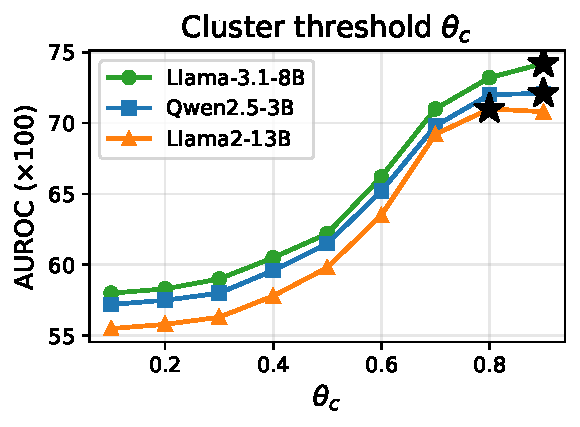
\includegraphics[width=0.32\textwidth]{resources/abl_theta_c}\hfill
  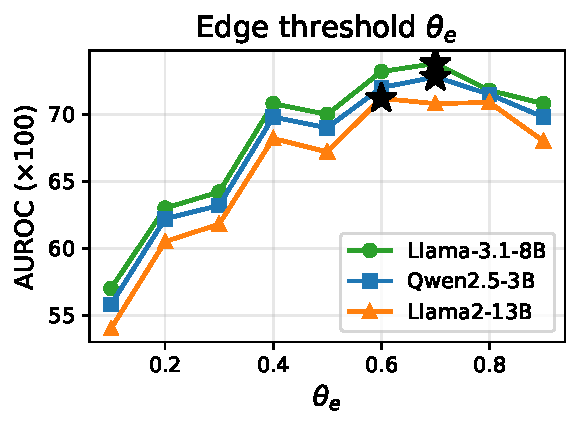
\includegraphics[width=0.32\textwidth]{resources/abl_theta_e}\hfill
  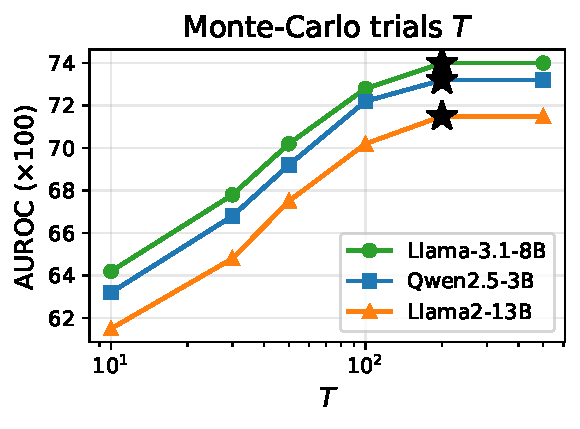
\includegraphics[width=0.32\textwidth]{resources/abl_T}
  \\[4pt]
  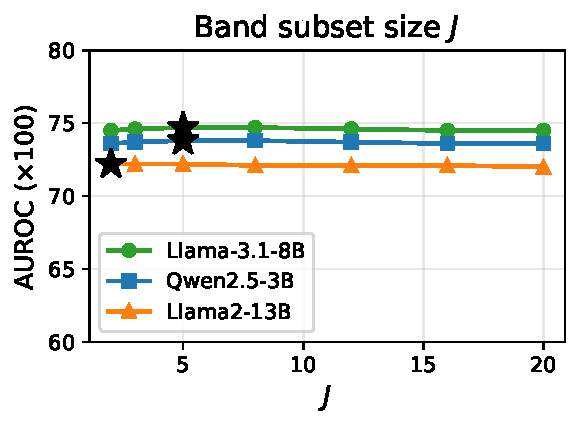
\includegraphics[width=0.32\textwidth]{resources/abl_J}\hspace{0.02\textwidth}
  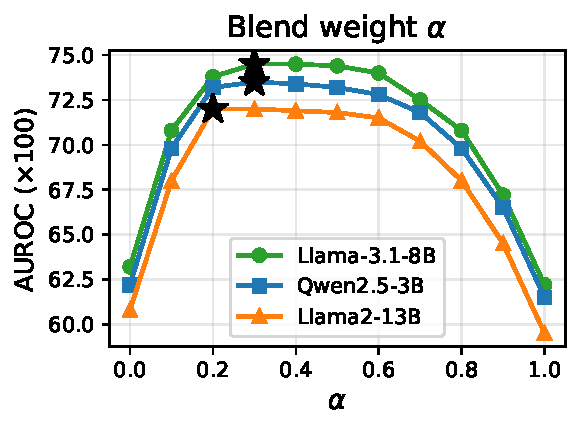
\includegraphics[width=0.32\textwidth]{resources/abl_alpha}
  \caption{gBD hyperparameter trends on SVAMP (each panel's title names the swept
  hyperparameter; $\star$ marks each model's best setting). The graph thresholds
  $\theta_c$ and $\theta_e$ and the trial count $T$ rise out of a degenerate
  low-resource regime and saturate onto a plateau; the subset size $J$ is flat; and
  the blend weight $\alpha$ peaks at an intermediate value before falling toward pure
  depth. The trends are consistent across the backbones we test.}
  \label{fig:ablation-trends}
\end{figure}

\subsection{Graph Construction Thresholds}
\label{sec:exp:ablation:thresh}

The reasoning graph depends on two cosine-similarity thresholds: the clustering
threshold $\theta_c$, above which two steps merge into a single node, and the
semantic-edge threshold $\theta_e$, above which steps from different chains are
joined by a soft edge. $\theta_c$ governs how aggressively the graph collapses
equivalent reasoning, and $\theta_e$ how densely the chains are cross-connected.
Both follow the rise-to-plateau pattern: at very low values the graph
degenerates---$\theta_c$ merges nearly all steps into one node and $\theta_e$ floods
the graph with spurious edges---so AUROC is poor, and it then improves and saturates
as the threshold sharpens. The defaults $\theta_c{=}0.92$ and $\theta_e{=}0.70$ lie
in the saturated region.

\subsection{Number of Monte-Carlo Trials}
\label{sec:exp:ablation:trials}

gBD approximates band depth by sampling $T$ pairs of random walks per estimate, so
small $T$ gives a noisy estimate at low cost and large $T$ a stable one at higher
cost. As $T$ grows the estimator variance shrinks and AUROC converges to a stable
value, beyond which further trials mostly add cost; the default $T{=}200$ sits at
the onset of this plateau.

\subsection{Confidence Blend Weight}
\label{sec:exp:ablation:alpha}

The final confidence blends band depth with the answer-level majority fraction
through $\alpha$ (Eq.~\eqref{eq:blend}), interpolating between pure majority vote
($\alpha{=}0$) and pure depth ($\alpha{=}1$). AUROC follows an inverted-U: it is
highest at an intermediate $\alpha$ and lower at either extreme, indicating that
reasoning-structure depth and answer agreement carry complementary information. The
default $\alpha{=}0.3$ lies near this interior optimum, and we keep a single
per-method $\alpha$ across all benchmarks rather than tuning per dataset.

\section{Computational Complexity}
\label{app:complexity}

Table~\ref{tab:complexity} gives the per-question time and space complexity of each
method. $M$ is the ensemble size, $n$ the maximum chain length, $N \le Mn$ the total
number of steps, $d$ the embedding dimension, $|V|$ and $|E|$ the vertex and edge
counts of the reasoning graph, $S$ the number of sampled vertex subsets (vBD), $T$
the number of sampled reference-path subsets per chain (gBD), $J$ the band subset
size, and $\ell$ the length of a reference path. The graph cost is shared by vBD and
gBD and covers pairwise step similarities for clustering and semantic edges plus
all-pairs shortest paths.

\begin{table}[h]
  \caption{Per-question time and space complexity.}
  \label{tab:complexity}
  \centering
  \small
  \begin{tabular}{lll}
    \toprule
    \textbf{Method} & \textbf{Time} & \textbf{Space} \\
    \midrule
    Reasoning graph (vBD, gBD) & $O(N^2 d + |V|\,(|V| + |E|))$ & $O(N^2)$ \\
    \midrule
    pBD & $O(M^2 n^2 d)$ & $O(n^2 + Nd)$ \\
    vBD & $O(S J^2 |V|)$ & $O(|V|)$ \\
    gBD & $O(M T J^2 \ell^2 |V|)$ & $O(J\ell + |V|)$ \\
    \bottomrule
  \end{tabular}
\end{table}


\end{document}
